\section{Ejercicio 3: Búsqueda Local}
    % 1. Describir detalladamente el problema a resolver dando ejemplos del mismo y sus soluciones.
    \subsection{Descripción del problema y solución propuesta}

    \par Una vez obtenida una heurística greedy para resolver nuestra variante de TSP, utilizamos una \textbf{Búsqueda Local} para analizar una mayor cantidad de soluciones posibles. Es decir, dada una solución inicial S (obtenida de aplicar a una instancia de entrada, el algoritmo heurístico implementado en el Ejercicio 2) se obtienen los vecinos de S, es decir, un “vecindario“ de soluciones. Y de este vecindario, se obtiene el vecino cuya solución mejore a S. Luego se realiza una búsqueda local sobre este vecino. 
    \par Sea V este vecindario, $\forall S^{*}\in V, S^{*} = h(S)$. h es una función que obtiene un vecino a partir de S, perteneciente a V. En otras palabras, h altera la solución S para encontrar una solución parecida que pueda mejorar el resultado. Por otro lado, se cuenta con una función f que da valor a cada una de las soluciones. En nuestro caso, sean S y $S^{'}$, diremos que una solución S es mejor que $S^{'}$ si $f(S) < f(S^{'})$. Luego para cada $S^{*}\in V$, se evalúa f($S^{*}$). 
    \par Dado V el conjunto de vecinos del Vecindario y S la solución original, si $\forall S^{*}\in V, f(S) < f(S^{*})$  se devuelve la solución S. En caso contrario, se aplica nuevamente la búsqueda local sobre $S^{*}$ cuyo valor en f sea el menor, y se repite el procedimiento hasta que no haya un $S^{*}$ que cumpla $f(S^{*}) < f(S)$. Una vez que esto ocurre, se devuelve el último $S^{*}$. 
    \par De esta manera, a partir de una solución se estará explorando sus vecinos, y la búsqueda local se detendrá al hallar una mínimo local.

    \subsubsection{Vecindad A}

    \par Se realiza una búsqueda local aplicado a nuestro problema de la siguiente manera. La solución inicial S, se obtiene de aplicar la heurística del vecino más cercano (explicada en el Ejercicio 2) a los parámetros pasados por entrada. En nuestro caso, S consiste en una tupla con distancia, recorrido y cantidad de estaciones.
    \par Una vez obtenida esta solución, contamos con la función \textbf{h} la cual generará la primer vecindad. En este caso, la función $h$ se denomina \emph{dameVecindario}, y se encarga de intercambiar únicamente las \emph{pokeparadas} dentro del recorrido de S. Por cada intercambio generado, se guarda este nuevo recorrido en un vector.

    \begin{codesnippet}
    \begin{verbatim}
    vector<vector<int>> dameVecindario(lista<Estacion> estaciones, lista<int> recorrido)
        vector<vector<int>> vecindario;
        Para i = 0...recorrido.size() - 1
            Si la estacion pasada en el recorrido[i] no es gimnasio
                Para j = i+1 ... recorrido.size()
                    Si la estacion pasada en el recorrido[j] no es gimnasio
                        Creo un vector estadoAux <-- recorrido
                        Hago swap entre i y j en estadoAux
                        vecindario.push_back(estadoAux);
                    Fin si
                Fin
            Fin Si
        Fin
        Devolver vecindario
    \end{verbatim}
    \end{codesnippet}

    En nuestro caso, una solución es mejor que otra si una logra conquistar todos los Gimnasios recorriendo menor distancia que la otra, manteniendo siempre el invariante de no pasar por la misma estación más de una vez. 
    Una vez obtenido el vecindario, la función f evalúa cada solución. En nuestro caso f se llama “dameDistancia“ y se encarga de calcular la distancia de cada solución obtenida, guardándola en el vector vecindario. Luego compara cada una con S. 
    \par Si la distancia de algún recorrido nuevo en el vecindario (por ejemplo $S^{'}$) es menor que la distancia que recorrió S, se repite el ciclo de búsqueda local sobre algún $S^{'}$. Caso contrario, se devuelve la solución S con su recorrido, su distancia y la cantidad de estaciones por donde pasó.

   \subsubsection{Vecindad B}

    \par A diferencia de la Vecindad A, la función h del vecindario B, se llama “dameVecindario2“ y se encarga de intercambiar únicamente los \emph{gimnasios} dentro del recorrido S, siempre que cada intercambio de gimnasios en el recorrido no cause que alguno de los gimnasios no pueda ser conquistado.

    \begin{codesnippet}
    \begin{verbatim}
    vector<vector<int>> dameVecindario2(lista<Estacion> estaciones, lista<int> recorrido,
                                        matriz<double, double> distancias, int k)
        vector<vector<int>> vecindario;
        Para i = 0...recorrido.size() - 1
            Si la estación pasada en el recorrido[i] es gimnasio
                Para j = i+1 ... recorrido.size()
                    Si la estación pasada en el recorrido[j] es gimnasio
                        Creo un vector estadoAux <-- recorrido
                        Hago swap entre i y j en estadoAux
                        Si el recorrido sigue siendo válido (se conquistan todos los gimnasios)
                            vecindario.push_back(estadoAux);
                        Fin si
                    Fin si
                Fin
            Fin Si
        Fin
        Devolver vecindario
    \end{verbatim}
    \end{codesnippet}
    
    \par El resto del procedimiento es equivalente al explicado para la búsqueda local que incluye el Vecindario A.
   
    \subsection{Complejidad teórica}
        Para la complejidad teórica, debemos mostrar por cada iteración de la búsqueda local cual será la cota asintótica. 
        \par Para empezar, hablaremos de la \textbf{Vecindad A}. Como fue explicado anteriormente, se encarga de crear las posibles combinaciones de intercambiar la posición de las pokeparadas en el recorrido. Para calcular la complejidad en cada iteración de la búsqueda local, sean N los nodos gimnasio y M los nodos pokeparadas, se deben tener en cuenta:

        \begin{itemize}
            \item Para ingresar a la búsqueda local, se copia el vector recorrido, de la solución inicial S, esto cuesta \ord(N+M).
            \item Luego se entra al ciclo principal de búsqueda local que en el peor de los casos tendrá M! iteraciones. Esto se debe a que, dado que en cada iteración se permutan ciertas pokeparadas, en el peor de los casos, siempre encuentra una solución mejor. Va a tomar \ord(M!) iteraciones recorrer todas las permutaciones posibles.
            \item Dentro del ciclo principal, se busca el vecindario de una solución. Para esto se llama a la función \emph{dameVecindario} con el vector \emph{recorrido}.
            La misma función, recorre el vector hasta que el i-ésimo elemento sea pokeparada. Luego recorre el vector restante, desde i+1 hasta recorrido.size()-1. Es decir, la complejidad del ciclo, siendo r la cantidad de estaciones del recorrido, es de 
            \[
            \ord(\sum_{i=0}^{r-1} i)
            \] 
            
            \par Que dada la progresión aritmética,
            \[
            \sum_{i=0}^{r-1} i = r * (r - 1)
            \]

            \par Esto quedaría,
            \[
            \ord(r * (r - 1) / 2)
            \]
            \par Además, como mencionamos anteriormente, el tamaño del recorrido en el peor caso es \ord(N+M). Luego,
            \[
            \ord((N+M))*(N+M-1)/2)
            \]

            Luego, dentro del ciclo, se copia el vector recorrido en un vector \emph{estadoAux}, la copia del vector es \ord(N+M), y si esto se realiza en cada ciclo,
             \[
            \ord(((N+M))*(N+M-1)/2)*(N+M)) = \ord((N+M)^{3})
            \]

            \item Una vez obtenido el vecindario se recorre el vector \emph{vecindario} y por cada vecino se itera sobre su recorrido calculando la distancia. Dado que las iteraciones dentro de \emph{dameVecindario}, empieza en la i-ésima pokeparada, y por cada elemento a partir del i+1, que también sea pokeparada, se genera un intercambio de elemento dentro del vector, entonces la cantidad de vecinos distintos serán,
            \[
             $\sum_{i=0}^{M-1} i = M(M-1)/2$
            \] 
            Luego la cantidad de vecinos diferentes, es decir el tamaño total del vector vecindario es de $M(M-1)/2$. Calcular la distancia, implica por cada vecino, recorrer todo el vector \emph{recorrido}, esto es \ord(N+M). Esto lo realiza para los M(M-1)/2 vecinos. Es decir
            \[
                \ord((M(M-1)/2)*(N + M)) = \ord(M^{2}*(N+M))
            \]
            \item Finalmente, dada la solución, se genera una tupla en \ord(1) y se devuelve esta solución.

        \end{itemize}

        Es decir, la complejidad quedaría
        \[
            \ord(N+M) + \ord(M!)*(\ord((N+M)^{3}) + \ord(M^{2}*(N+M)) =
        \]
        \[
            \ord(M!)*(\ord((N+M)^{3}) + \ord(M^{2}*(N+M)) =
        \]
        \[
            \ord(M!*((N+M)^{3} + M^{2}*(N+M))) =
        \]

        \[
            \ord(M!*((N+M)^{3}))
        \]
        Pues $\ord(M^{2}*(N+M)) = \ord((N+M)^{3})$

        Finalmente, la complejidad total es de
        \[
            \ord(M!*((N+M)^{3}))
        \] 


        \par Por otro lado, hablaremos de la complejidad del vecindario B. La misma, comparte gran parte de la complejidad del vecindario A. Por lo que se nombrarán las partes relevantes del algoritmo de búsqueda local con el vecindario B.
        \begin{itemize}
            \item Para ingresar a la búsqueda local, se copia el vector recorrido, de la solución inicial S, esto cuesta \ord(N+M).
            \item Luego, busca las permutaciones de los gimnasios, por lo que, el ciclo principal de la búsqueda local, tendrá en el peor de los casos N! iteraciones. Es decir, si intercambiar los gimnasios siempre genera una solución posible, como en cada iteración se permutan algunos gimnasios, en el peor de los casos, siempre encuentra una solución mejor dentro del vecindario. Luego esto tomará \ord(N!) iteraciones recorrer todas las permutaciones posibles.
            \item Dentro del ciclo principal, se busca el vecindario de la solución. Para esto, se llama a la función \emph{dameVecindario2} con el vector \emph{recorrido}. Hace las mismas iteraciones que en el vecindario A, es decir 
            \[
                \ord((N+M)*(N+M-1)/2)
            \]

            Con la diferencia que, sea r = recorrido.size(), copiar el vector\emph{recorrido} en \emph{estadoAux} cuesta \ord(r), y además debe chequear que el nuevo recorrido es válido. Para esto, recorre nuevamente el vector \emph{estadoAux}, viendo que se cumplan diferentes condiciones. Luego como fue mencionado, dado que se copia \emph{recorrido} en \emph{estadoAux} y $r = \ord(N + M)$, entonces $estadoAux.size() = r = \ord(N+M)$. Luego copiar el vector es \ord(N+M) y recorrer el vector estadoAux, es 
            \[
                \ord(2*(N+M)) = \ord(N+M)
            \]

            Esto quiere decir que, por cada ciclo de \emph{dameVecindario2}, debe copiar el vector y chequear que sea válido. Y las iteraciones de esta función eran \ord((N+M)*(N+M-1)/2). Luego quedaríá \ord((N+M)*(N+M-1)/2*(N+M)), entonces
            \[
                \ord((N+M)*(N+M-1)/2*(N+M)) = \ord((N+M)^3)
            \]

            \item Luego una vez obtenido el vecindario, se calcula al igual que en el \textbf{vecindario A} las distancias de cada vecino en $\ord(M^{2} * (N+M))$
            \item Por último en $\ord(1)$ se genera una tupla como solución y se devuelve.

            Entonces, la complejidad quedaría
        \[
            \ord(N+M) + \ord(N!)*(\ord((N+M)^{3}) + \ord(M^{2}*(N+M)) =
        \]
        \[
            \ord(N!)*(\ord((N+M)^{3}) + \ord(M^{2}*(N+M)) =
        \]
        \[
            \ord(N!*((N+M)^{3} + M^{2}*(N+M))) =
        \]
        \[
            \ord(N!*((N+M)^{3}))
        \]
        Pues $\ord(M^{2}*(N+M)) = \ord((N+M)^{3})$

        Finalmente, la complejidad total es de
        \[
            \ord(N!*((N+M)^{3}))
        \] 

        \end{itemize}
    % 4. Dar un código fuente claro que implemente la solución propuesta. Se deben incluir las partes relevantes del código como apéndice del informe impreso entregado.

    \subsection{Detalles Implementativos}

    
    Las clases y estructuras utilizadas en el algoritmo son las mismas que las del primer ejericio. El algoritmo propuesto para las búsquedas locales es el siguiente: 

            \begin{codesnippet}
            \begin{verbatim}

solucion busquedaLocal(vector<int> recorridoInicial, vector<Estacion> estaciones, 
    matriz<double> distancias, double distancia, bool elegirVecindario)
    
    matriz<int> vecindario;
    double distanciaMinima;
    double distanciaAux;
    int proximoEstado;
    bool hayanSoluciones = true;
    vector<int> recorrido = recorridoInicial;

    mientras hayanSoluciones
        vecindario = dameVecindario(estaciones, recorrido, elegirVecindario)
        //obtiene un vecindario de soluciones
        
        proximoEstado = -1;

        si el vecindario no es vacio
            
            distanciaMinima = distancia;
            
            //Busco algun vecino con distancia mas chica
            para cada vecino entre 0 y tam(vecindario)
                
                distanciaAux = dameDistancia(vecindario[vecino], distancias);
                //obtiene las distancia recorridas de la solucion vecino-ésima

                si distanciaAux < distanciaMinima
                    distanciaMinima = distanciaAux;
                    proximoEstado = vecino;
                fin si
            fin para cada
        fin si
    
        si proximoEstado > -1
            recorrido = vecindario[proximoEstado];
            distancia = distanciaMinima;
        sino
            hayanSoluciones = false;
        fin si

    fin mientras

    devolver solucion (distancia, tam(recorrido), recorrido);
fin busquedaLocal
            \end{verbatim}
            \end{codesnippet}


            El algoritmo obtiene una primera solución \textbf{recorridoInicial} en base al algoritmo greedy goloso implementado en el Ejercicio 2.
            \par Luego, busca un vecindario de soluciones en base a la solución obtenida (dado el parámetro \textbf{elegirVecindario}, se elige uno de los dos tipos de vecindarios).
            \par Se obtiene la mejor solución del vecindario, es decir, la que menor distancia recorre. Llamémosla S.
            \par Por último se vuelve a repetir el procedimiento, buscando un vecindario de soluciones a partir de la solución S.

            \par Todo este procedimiento se repite hasta que el vecindario de soluciones no contenga ninguna solución mejor que la solución ya obtenida.


    % 5. Realizar una experimentación computacional para medir la performance del programa implementado. Usar un conjunto de casos de test en función de los parámetros de entrada, con instancias aleatorias e instancias particulares (de peor/mejor caso en tiempo de ejecución, por ejemplo). Presentar en forma gráfica una comparación entre los tiempos medidos y la complejidad teórica calculada y extraer conclusiones.
    \subsection{Experimentación}
    Los experimentos realizados permiten observar las diferentes calidades de solución para ambos vecindarios, es decir, se comparó junto al resultado exacto dado por backtracking, qué vecindario devolvía la menor distancia posible. Como hipótesis mantuvimos que, dado que en el vecindario A se intercambian pokeparadas, el campo de soluciones recorridas por él es mayor al del vecindario B, debido a que, al intercambiar pokeparadas de una solución esta sigue siendo solución, mientras que en el vecindario B, por cada intercambio de gimnasios, debe filtrar aquellos que no devuelven una solución válida, teniendo menos margen para generar vecinos. Entonces, \textbf{en general}, esto permite que el vecindario A, obtenga mejores soluciones que el B. Además se comparó la performance de cada vecindario.

        \subsubsection{Experimento 1: Calidad de resultado} 
            Para experimentar acerca de la calidad de los resultados de ambas vecindades, se generaron distintas comparaciones. 

            \begin{itemize}
                \item Por un lado, se comparó cada vecindario por separado con backtracking. Para esto se generaron 66 instancias, de las cuales, las primeras 20 instancias cumplen las mismas condiciones mencionadas en \textbf{Ejercicio 1: Experimento 1}. Por otro lado las siguientes 16 instancias  cumplen con las mismas condiciones que menciona el \textbf{Ejercicio 1: Experimento 2} y por último, fueron generadas 30 instancias arbitrarias.
 
                \item Por otro lado, se compararon los tres algoritmos juntos, corriendo 16 instancias creadas también manualmente. Por cada instancia, aumentamos de la misma manera la cantidad de gimnasios, pokeparadas y capacidad de las mochilas. Manteniendo siempre que la distancia entre cada estacion es 1.
            \end{itemize}

             En ambas comparaciones, por cada algoritmo, se corrió 30 veces la misma instancia, sacando un promedio de la distancia devuelta. Luego, en función de la cantidad de estaciones (n+m), se comparó qué distancias devolvían.

\blindtext

\begin{figure}[H]
\minipage{0.5\textwidth}
  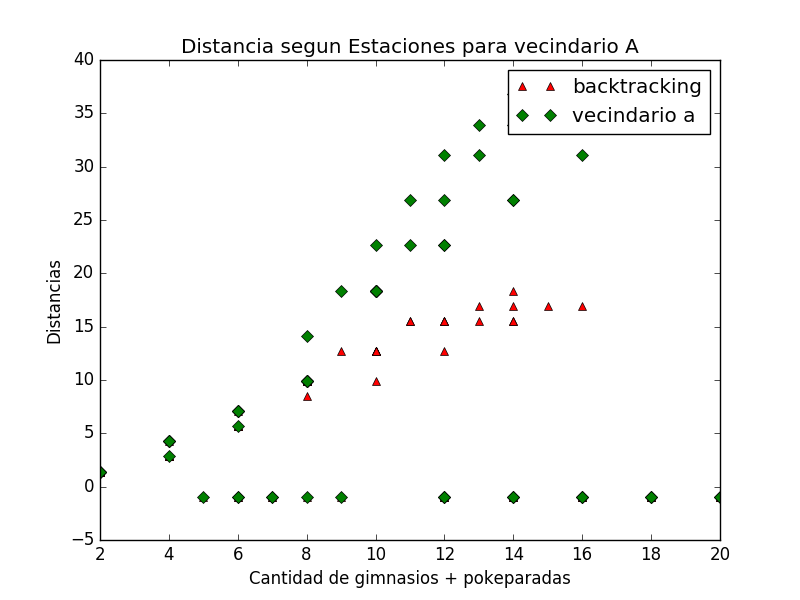
\includegraphics[width=\linewidth]{imagenes/Exp2Ej3A.png}
  \caption{Vecindario A}
\endminipage\hfill
\minipage{0.5\textwidth}%
  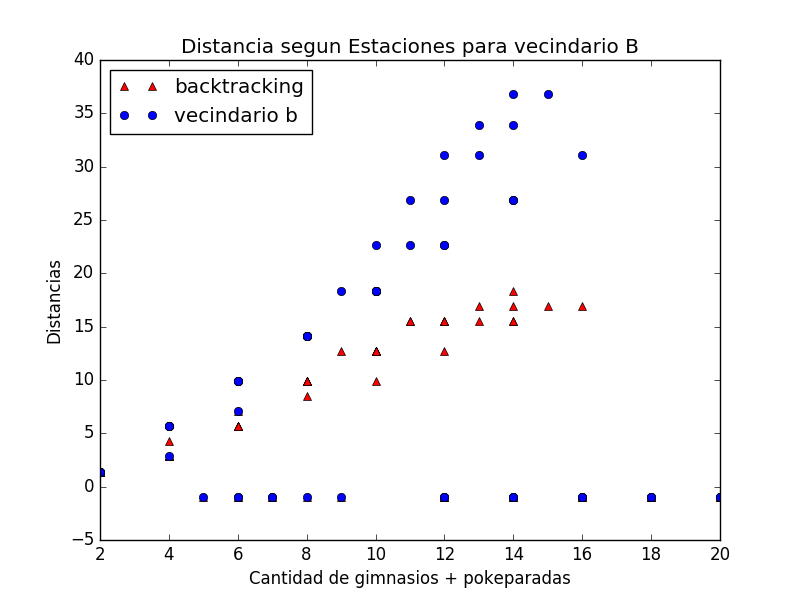
\includegraphics[width=\linewidth]{imagenes/Exp2Ej3B.png}
  \caption{Vecindario B}
\endminipage
\end{figure}

\blindtext

Para estas instancias, se puede observar que a medida que crece la cantidad de estaciones, crece la brecha entre la solución heurística con búsqueda local, y la solución exacta con backtracking. Esto se debe principalmente a que, a mayor cantidad de estaciones, el campo de soluciones crece. Es decir, mientras que backtracking recorre absolutamente todo el campo de soluciones obteniendo un mínimo global, la búsqueda local a partir de un resultado, recorre únicamente sus vecinos, deteniéndose en los mínimos locales. 

\par Luego dado el vecindario A, se observa que para instancias chicas, las soluciones se asemejan a las exactas pero sus distancias empiezan a diferenciarse a partir de contar con 8 estaciones. Mientras que en el vecindario B, desde el primer momento Backtracking encuentra mejores soluciones. Esto nos convence de que  para ciertas instancias, intercambiar pokeparadas hace una mejor búsqueda en el vecindario de soluciones. 

Luego, como mencionamos, se compararon los resultados de ambos vecindarios juntos y el resultado exacto.

  \begin{figure}[H]
      \begin{center}
        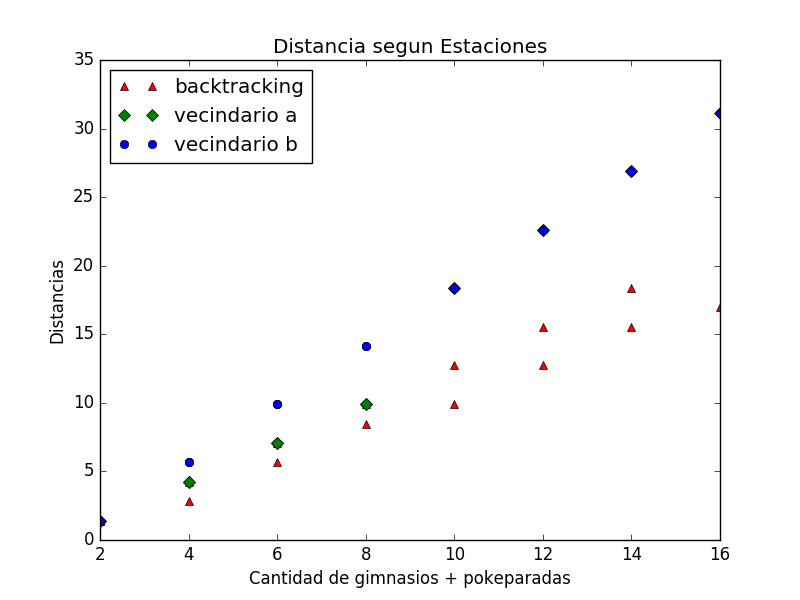
\includegraphics[width=0.7\columnwidth]{imagenes/Exp2Ej3TODO.png}
        \caption{Comparación vecindario y backtracking}
      \end{center}
  \end{figure}


Para este caso, se usaron menos instancias para observar el comportamiento de los distintos vecindario en comparación con Backtracking.  Como se puede observar, para instancias chicas las distancias obtenidas por el vecindario A se asemejan a las de backtracking, es decir, a las soluciones exactas. Pero a medida que la cantidad de estaciones crecen, la brecha entre Backtracking y vecindario A crece. Esto mismo no sucede con el vecindario B, donde desde un principio mantiene una brecha creciente con el resultado exacto. Por lo tanto, afirma la hipótesis anteriormente mencionada.